\subsection{Princípio da demanda efetiva no médio prazo: um paradigma e duas alternativas?}
\label{Medium}

Até então, pode-se dizer que a teoria do crescimento liderado pela demanda enfrentava um dilema. Não conseguia conciliar estabilidade, distribuição funcional da renda exógena e grau de utilização da capacidade produtiva igual ao normal/planejado, aparentando uma trindade impossível do crescimento, conforme pode ser visto no diagrama \ref{diagrama}\footnote{Este diagrama é inspirado no ``trilema'' do crescimento apresentado por \textcite{cesaratto_neo-kaleckian_2015}.}.
Essa trindade impossível se mostrou falsa com o desenvolvimento do supermultiplicador sraffiano (SMS).


\begin{figure}[htb]
	\caption{Trindade ``impossível''}
	\label{diagrama}
	\begin{center}
		\resizebox{0.45\textwidth}{!}{%
			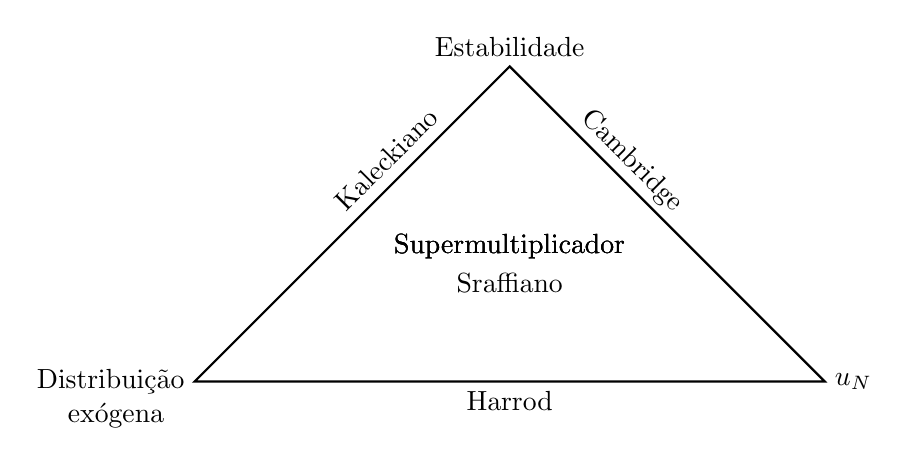
\begin{tikzpicture}[thick]
			\path[draw] (-4,0)  coordinate [label= left:Distribuição] (A)
			
			-- ( 0,4)  coordinate [label=above:Estabilidade] (C)
			-- ( 4,0)  coordinate [label=right:$u_N$] (B)
			-- cycle;
			\foreach \point in {A,B,C}
			\draw
			-- (0,2) node[anchor=north]{Supermultiplicador};
			\draw
			-- (-5,-0.15) node[anchor=north]{exógena};
			\draw
			-- (0,1.5) node[anchor=north]{Sraffiano};
			\draw
			-- (-1.75,3) node[anchor=north, rotate=45]{Kaleckiano};
			\draw
			-- (1.75,3) node[anchor=north, rotate=-45]{Cambridge};
			\draw
			-- (0,0) node[anchor=north]{Harrod};
			\end{tikzpicture}
		}
	\end{center}
	\caption*{\textbf{Fonte:} Elaboração própria}
\end{figure}
No entanto, da revisão da literatura verifica-se que tal mérito não se restringe ao SMS uma vez que uma vertente kaleckiana tem incluído tais gastos por meio do princípio do ajuste do estoque de capital no \textbf{longo prazo}.
Sendo assim, é possível avançar em direção a um mapeamento de uma possível convergência entre os modelos sraffianos do tipo supermultiplicador e os modelos kaleckianos e então selecionar o caminho a ser seguido (seção \ref{Concl1}).
Antes de prosseguir, no entanto, cabe destacar que por serem modelos na fronteira da literatura, podem não ser representativos do que se entende por modelo kaleckiano e, por conta disso, serão denominados ``não-tradicionais'' ao longo desta seção.


